\documentclass[supercite]{Experimental_Report}

\title{~~~~~~新生实践课~~~~~~}
\author{李嘉鹏}
\school{计算机科学与技术学院}
\classnum{CS2110}
\stunum{U202115652}
\instructor{陈加忠}
\date{2021年12月12日}

\usepackage{algorithm, multirow}
\usepackage{algpseudocode}
\usepackage{amsmath}
\usepackage{amsthm}
\usepackage{framed}
\usepackage{mathtools}
\usepackage{subcaption}
\usepackage{xltxtra} %提供了针对XeTeX的改进并且加入了XeTeX的LOGO, 自动调用xunicode宏包(提供Unicode字符宏)
\usepackage{bm}
\usepackage{tikz}
\usepackage{tikzscale}
\usepackage{pgfplots}
%\usepackage{enumerate}

\pgfplotsset{compat=1.16}

\newcommand{\cfig}[3]{
	\begin{figure}[htb]
		\centering
		\includegraphics[width=#2\textwidth]{images/#1.tikz}
		\caption{#3}
		\label{fig:#1}
	\end{figure}
}

\newcommand{\sfig}[3]{
	\begin{subfigure}[b]{#2\textwidth}
		\includegraphics[width=\textwidth]{images/#1.tikz}
		\caption{#3}
		\label{fig:#1}
	\end{subfigure}
}

\newcommand{\xfig}[3]{
	\begin{figure}[htb]
		\centering
		#3
		\caption{#2}
		\label{fig:#1}
	\end{figure}
}

\newcommand{\rfig}[1]{\autoref{fig:#1}}
\newcommand{\ralg}[1]{\autoref{alg:#1}}
\newcommand{\rthm}[1]{\autoref{thm:#1}}
\newcommand{\rlem}[1]{\autoref{lem:#1}}
\newcommand{\reqn}[1]{\autoref{eqn:#1}}
\newcommand{\rtbl}[1]{\autoref{tbl:#1}}

\algnewcommand\Null{\textsc{null }}
\algnewcommand\algorithmicinput{\textbf{Input:}}
\algnewcommand\Input{\item[\algorithmicinput]}
\algnewcommand\algorithmicoutput{\textbf{Output:}}
\algnewcommand\Output{\item[\algorithmicoutput]}
\algnewcommand\algorithmicbreak{\textbf{break}}
\algnewcommand\Break{\algorithmicbreak}
\algnewcommand\algorithmiccontinue{\textbf{continue}}
\algnewcommand\Continue{\algorithmiccontinue}
\algnewcommand{\LeftCom}[1]{\State $\triangleright$ #1}

\newtheorem{thm}{定理}[section]
\newtheorem{lem}{引理}[section]

\colorlet{shadecolor}{black!15}

\theoremstyle{definition}
\newtheorem{alg}{算法}[section]

\def\thmautorefname~#1\null{定理~#1~\null}
\def\lemautorefname~#1\null{引理~#1~\null}
\def\algautorefname~#1\null{算法~#1~\null}

\begin{document}
	
	\maketitle
	
	\clearpage
	
	\pagenumbering{Roman}
	
	\tableofcontents[level=2]
	\clearpage
	
	\pagenumbering{arabic}
	
	\section{网页整体框架}
	
	图\ref{fig1-1}是我的网页整体框架。
	
	\begin{figure}[htb] % here top bottom
		\begin{center}
			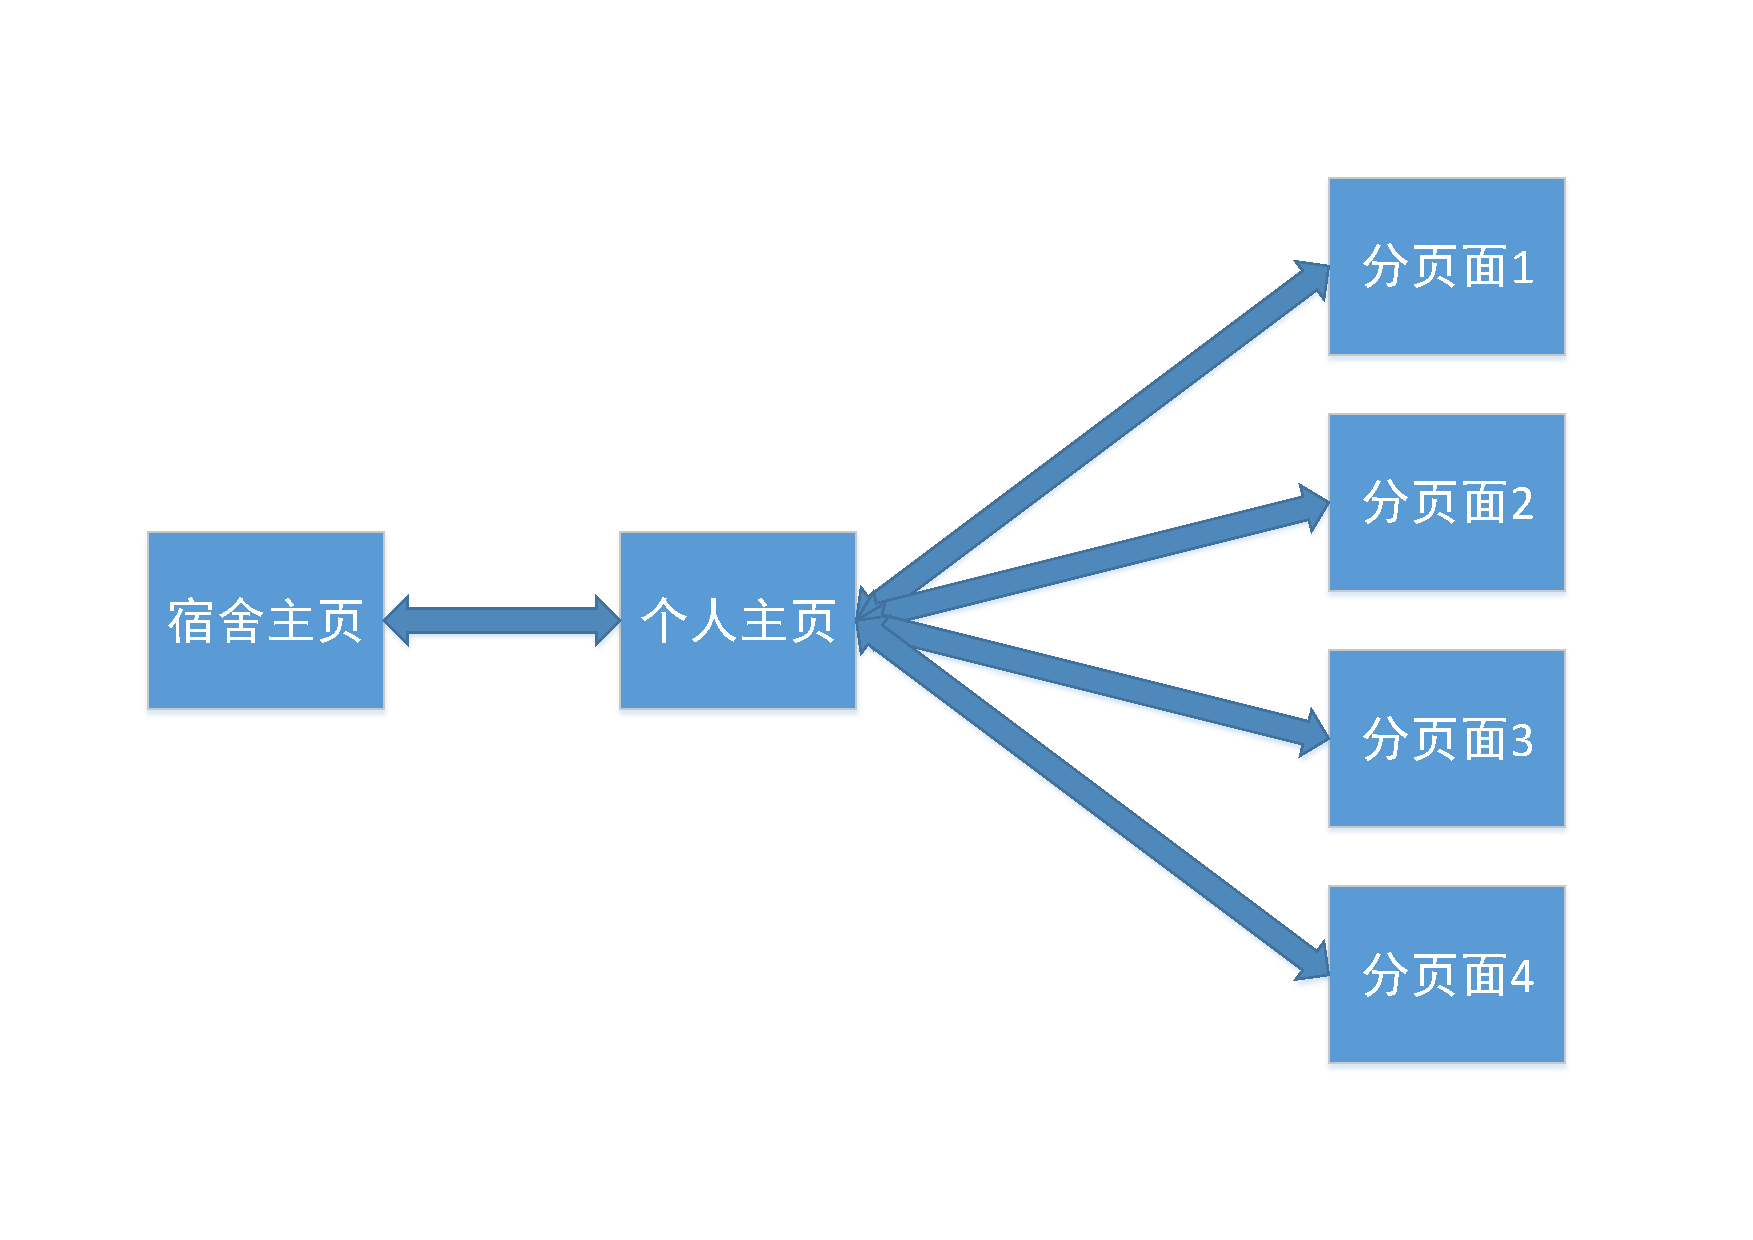
\includegraphics[scale=0.50]{images/1-1.pdf}
			\caption{网页整体框架}
			\label{fig1-1}
		\end{center}
	\end{figure}
	
	
	我的新生实践课网页总共由5个页面组成。其中,我的个人主页(index.html)为其余四个子页面(web1.html、web2.html、web3.html和web1.html)的主页。
	
	每个子页面都可通过特定的链接返回主页,同时,通过主页也能分别进入各个子页面。主页还能返回我们宿舍的主页,通过宿舍主页也能进入我的个人主页。
	
	\newpage
	
	\section{主页设计}
	
	我的主页是前往四个分页面的入口,其中包含了新生实践课网页设计作业的大标题、我的姓名、班级和学号等信息。同时,按2×2的格式列出了四个分页面的链接,并在这四个链接上方的中间位置设置了返回寝室主页的链接,方便查看与不同页面间的跳转。
	
	请见下图\ref{fig2-1}。
	
	\begin{figure}[htb]
		\begin{center}
			
\includegraphics[scale=0.50]{images/2-1.jpg}
			\caption{主页}
			\label{fig2-1}
		\end{center}
	\end{figure}
	
	在设计主页时,我希望能够将其变得清晰明了,方便使用。因此,我以一张优美的风景照作为主页背景,使整个画面既整洁又明亮,提升了页面的视觉效果。为了方便老师评分,我在主页上标注了个人信息,以期减少老师查阅我的信息的时间。在这些信息之下,我分别放置了四个分页面的入口,分别是:网页1(某公司官网)、网页2(班级支部网站)、网页3(个人观影网站)以及网页4(点歌台),让人能迅速地知晓网页的大概内容,并进入对应的页面进行查看。
	\newpage
	
	\section{分页面设计}
	
	我的主页总共包含4个分页面,它们分别取材于不同的主题和内容,检验并提高了我的网页实际制作能力。下面,我将一一对其进行分析。
	
	\subsection{某公司官网}
	
	本页面的截图如下图\ref{fig3-1}、图\ref{fig3-2}。
	
	\begin{figure}[htb]
		\begin{center}
			
\includegraphics[scale=0.43]{images/3-1.jpg}
			\caption{页面1截图1}
			\label{fig3-1}
		\end{center}
	\end{figure}

    \begin{figure}[htb]
    	\begin{center}
    		
\includegraphics[scale=0.43]{images/3-2.jpg}
    		\caption{页面1截图2}
    		\label{fig3-2}
    	\end{center}
    \end{figure}
	
	该页面顶端包含列表、方案、开发、返回主页和搜索等常用功能。在顶端菜单的下方,我放置了某公司新手机宣传片的截图,并在下方配以文字说明,让网站的来访者及时接收到最新产品消息。页面底部是该公司最近的新闻与动态,左侧置有“News”的图标,右侧用大字号写清了新闻的标题和时间,使网页具有很强的时效性。
	
    此页面中,为了使背景变为我选中的图片,我使用了代码\ref{alg:1}。
    
    为了让“返回主页”按钮发挥作用,需要使用超链接代码\ref{alg:2}。
    
    出于美观的需要,我需要使所有文字都位于画面的中央,这可以利用代码\ref{alg:3}实现。
	
	\begin{shaded*}\begin{alg}{页面背景自定义}
			\label{alg:1}
			\begin{algorithmic}
			<body background="../image/bg.jfif">
			
			<tbody>
			\end{algorithmic}
	\end{alg}\end{shaded*}

	\begin{shaded*}\begin{alg}{返回主页}
			\label{alg:2}
			\begin{algorithmic}
				<td width="155" bgcolor="#000000"><blockquote>
				
				<p><a href="../index.html" target="self"><strong>...</strong></a></p>
				
				</blockquote></td>
			\end{algorithmic}
	\end{alg}\end{shaded*}

    \begin{shaded*}\begin{alg}{文字居中}
    		\label{alg:3}
    		\begin{algorithmic}
    			text-align: center;
    		\end{algorithmic}
    \end{alg}\end{shaded*}
	
	\subsection{班级支部网站}
	
	本页面的截图如下图\ref{fig3-3}。

	\begin{figure}[htb]
		\begin{center}
			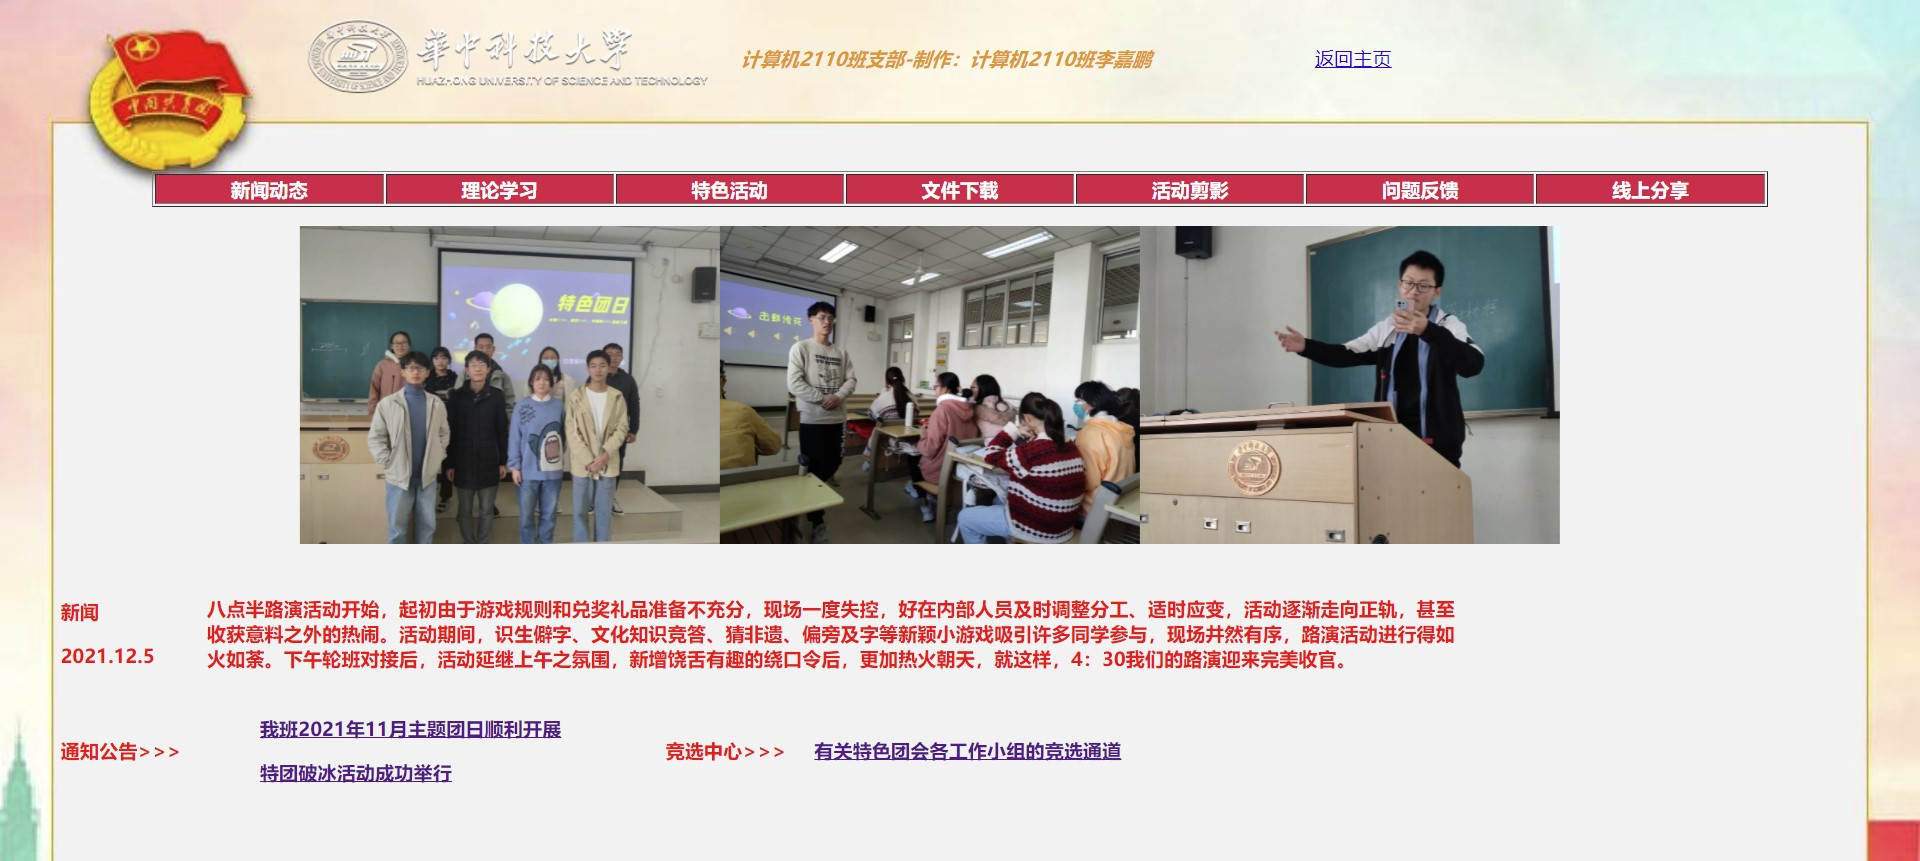
\includegraphics[scale=0.40]{images/3-3.jpg}
			\caption{页面2截图}
			\label{fig3-3}
			\end{center}
	\end{figure}
	
	这个页面主要是联系班级团支部实际情况而设计的。页面以红色为基调,上方有华中科技大学校徽与logo,附带写有我的姓名。右侧是“返回主页”的超链接。
	
	在下方,有一行菜单用于功能选择。它们分别为“新闻动态”“理论学习”“特色活动”“文件下载”“活动剪影”“问题反馈”和“线上分享”,涵盖了一个此类网站所需的全部功能。
	
	在此之下有三张实时循环滚动的图片,使整个页面更加鲜活生动。再往下是最近新闻及其内容、通知公告以及竞选中心,其中后两项都带有超链接,方便进入外部页面。
	
	其中滚动图片的代码实现如下\ref{alg:4}。
	
	\begin{shaded*}\begin{alg}{图片滚动}
			\label{alg:4}
			\begin{algorithmic}
				<marquee>
				
				<p>
				
				<img src="../image/2-1.jpg" width="350" height="265" alt=""/>
				
				<img src="../image/2-2.jpg" width="350" height="265" alt=""/>
				
				<img src="../image/2-3.jpg" width="350" height="265" alt=""/>
				
				</p>
				
				</marquee>
			\end{algorithmic}
	\end{alg}\end{shaded*}
	
	\subsection{个人观影网站}
	
	本页面的截图如下图\ref{fig3-4}。
	
	\begin{figure}[htb]
		\begin{center}
			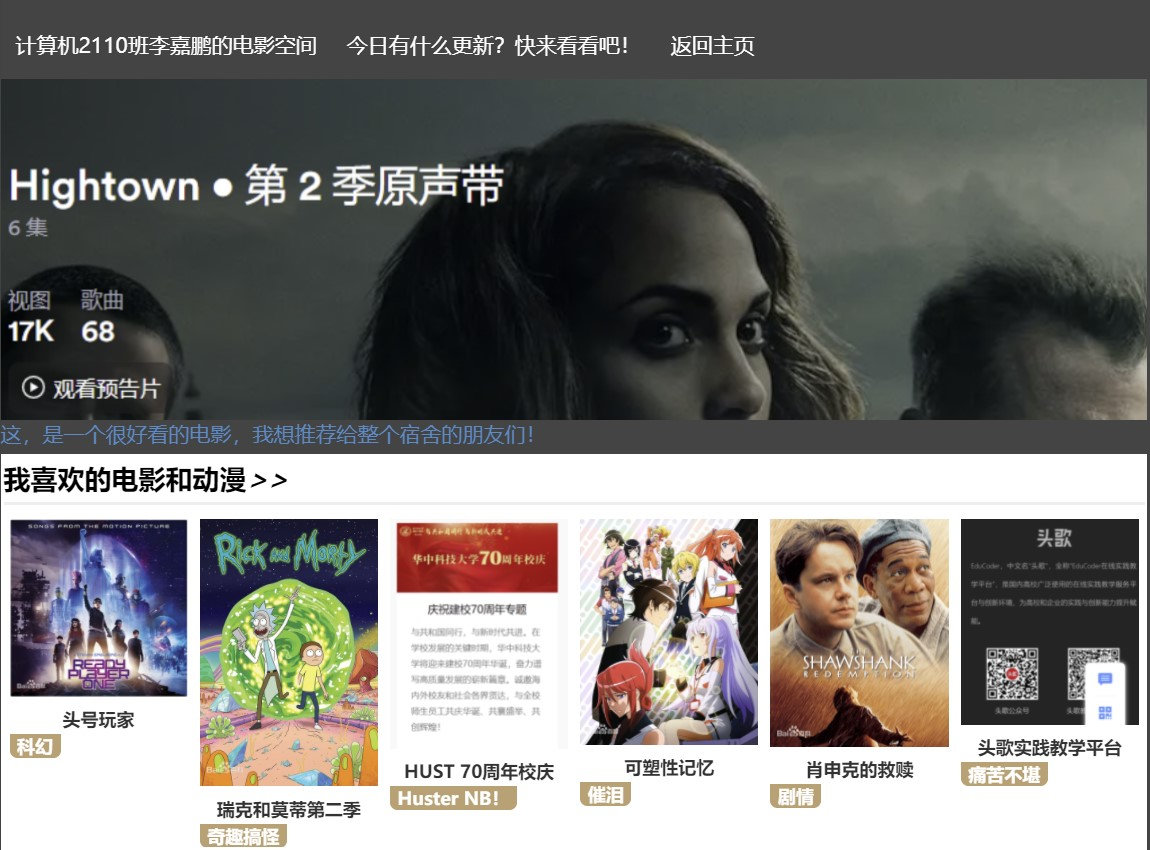
\includegraphics[scale=0.50]{images/3-4.jpg}
			\caption{页面3截图1}
			\label{fig3-4}
		\end{center}
	\end{figure}

	该页面的灵感来源是平时在线观看电影的平台,我尽可能复原了一个观影网站的外观。
	
	在此页面的顶端是一个功能条,分别写有“计算机2110班李嘉鹏的电影空间”“今日更新”以及“返回主页”的链接。功能条下方是一个首页展示窗,用来放置推荐电影的大图,为其留出独立空间吸引观众注意。再往下是“我喜欢的电影和动漫”板块,包含一些影视作品的名称、宣传图和分类。
	
	此页面中,我加入了一些动画视觉效果。值得注意的有两点:其一是当鼠标移至最上面的功能条时,对应的按钮会由灰色变为白色,如图\ref{fig3-5}。
	
	\begin{figure}[htb]
		\begin{center}
			
\includegraphics[scale=1.20]{images/3-5.jpg}
			\caption{页面3截图2}
			\label{fig3-5}
		\end{center}
	\end{figure}
	
	其二是当鼠标移至下方具体的影视作品上时,对应的图片会产生立体边框,如图\ref{fig3-6}。

    \begin{figure}[htb]
    	\begin{center}
    		
\includegraphics[scale=1.3]{images/3-6.jpg}
    		\caption{页面3截图3}
    		\label{fig3-6}
    	\end{center}
    \end{figure}
	
	
	\subsection{点歌台}
	
	本页面的截图如下图\ref{fig3-7}。
	
	\begin{figure}[htb]
		\begin{center}
			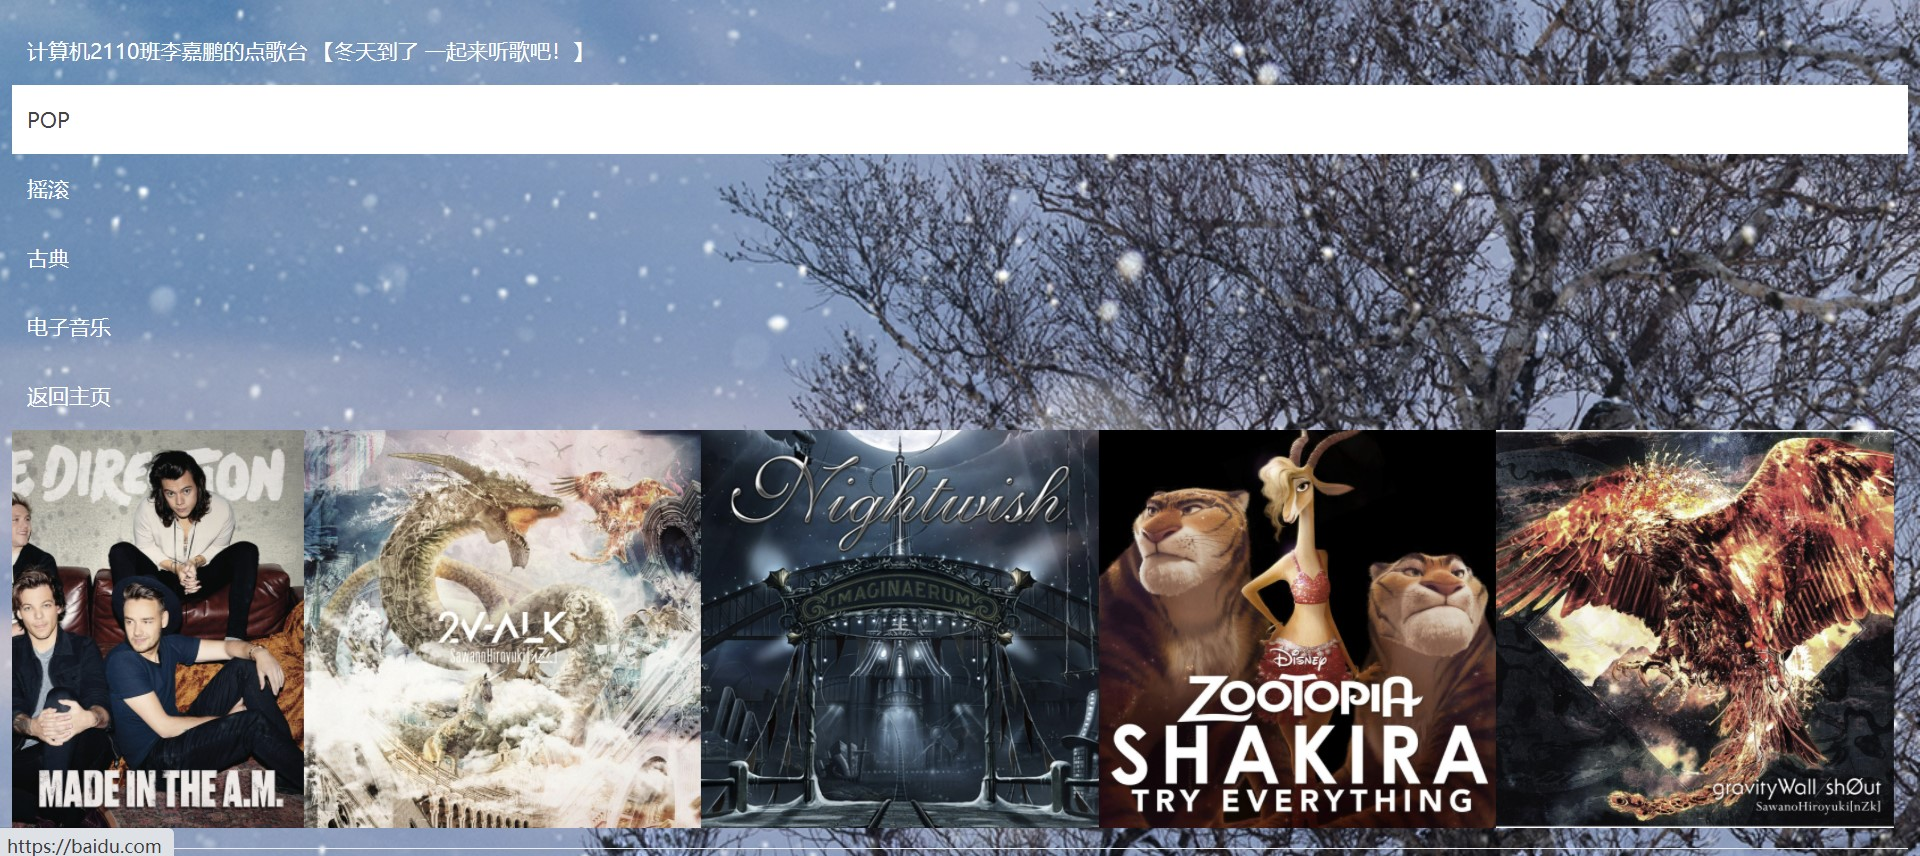
\includegraphics[scale=0.43]{images/3-7.jpg}
			\caption{页面4截图}
			\label{fig3-7}
		\end{center}
	\end{figure}
	
	该页面的灵感来源于各大音乐平台的网页播放器。
	
	在这个页面中,我将页面3中的横向功能条改为了纵向,增大了用户操作的空间。同时,我也再次借用了此前提到的图片滚动功能,使页面具有音乐播放器的特色。
	
	\newpage
	
	\section{网页设计小结}
	
	经过几周的不懈努力,网页设计终于告一段落。
	
	作为一名初学者,我在网页设计的探索过程中曾经遇到了许多困难,例如:在开始阶段,不知道怎样调节字体、字号、颜色、居中等文字格式,不懂得如何让界面更加美观、操作方便,也不清楚怎样实现页面中更高级的功能。不过,在反复的练习和同学的帮助之下,我终于掌握了文字格式的调整;通过观摩众多成熟的网站,对相关的美术版面设计、UI界面设计等细节有了更加深刻的理解;同时,通过自学网上社区内的相关知识,我也能逐渐打磨出自己的高级功能,实现了网页制作水平的飞跃。
	
	因此,这次网页设计是我的一次十分宝贵的学习经验。它不仅提高了我的眼界,丰富了我的网页制作经验,也培养了自学和试错能力,让我受益匪浅。
	
	\newpage
	
	\section{课程的收获和建议}
	
	通过新生实践课的学习,我对众多软件的使用都有了比较深的了解,为我以后的学习生活打下了坚实的基础。例如在论文编辑工具LaTex对我未来发布文章、实验报告等都具有不可替代的作用;通过对Python的学习,让我了解了一种新的语言及其特点,增长了作为计算机学生的我的见识;又如对Photoshop及Dreamweaver软件的学习,让我在图片编辑、网页制作等领域上掌握了更好的技能。
	
	总之,这门课程让我学习到了很多实际的、应用性的知识,对我帮助很大。
	
	\subsection{计算机基础知识}
	
	这一专题的学习中,我进一步了解了计算机的发展历程及规律、计算机系统的结构和组成,学习了冯·诺依曼结构框图和计算机硬件的组成部分(如主板、总线、CPU、内存、外存等)。不仅如此,我还对数据在计算机中的表现形式(二进制及其逻辑、运算规则)有了更透彻的理解,进一步分析了计算机的运作方式。
	
	\subsection{文档撰写工具LaTeX}
	
	这一专题中我认识了一个非常优秀的排版软件,学习了许多编辑文章的实用技能,包括:
	
	\begin{enumerate}
		\renewcommand{\labelenumi}{\theenumi)}
		\item LaTex的基本语句格式、命令、文档类型、宏包、环境等要素
		\item 修改文章作者、标题、摘要、目录、文字格式(字号、字样、字间距等)、参考文献的方法
		\item 插入表格、数学公式、图片的方法
	\end{enumerate}
	
	运用这些知识,我完成了一些任务,例如图\ref{fig4-1}、\ref{fig4-2}。
	
	\begin{figure}[htb]
		\begin{center}
			
\includegraphics[scale=0.8]{images/4-1.jpg}
			\caption{替换文字内容}
			\label{fig4-1}
		\end{center}
	\end{figure}

    \begin{figure}[htb]
    	\begin{center}
    		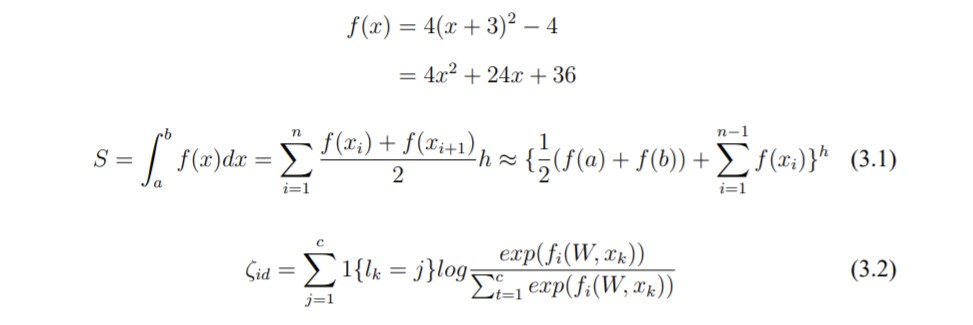
\includegraphics[scale=0.8]{images/4-2.jpg}
    		\caption{插入数学公式}
    		\label{fig4-2}
    	\end{center}
    \end{figure}
	
	我相信,这将会在我以后写报告或论文时提供极大的帮助!
	
	\subsection{编程工具Python}
	
	通过对Python的学习,我认识了一种全新的可读性强、应用范围广泛、面向对象的编程语言。通过课上的例子,我学会了如何安装Python开发环境、配置解释器,以及其基础语法、数据类型、表达式、函数结构与流程控制,增强了我利用Python解决实际问题的能力,丰富了我的编程经验。
	
	\subsection{图像设计软件Photoshop}
	
	在这个专题的学习中,我首先学习了Visio这一绘制流程图和示意图的软件,了解了如何通过画图的方式处理复杂的数据和信息。
	
	然后,学习完Photoshop后,我了解了它的各项菜单、功能所在位置,以及其中诸多功能如何使用,包括:
	
	\begin{enumerate}
		\renewcommand{\labelenumi}{\theenumi)}
		\item 仿制图章、图案图章、修复等功能
		\item 画笔工具和铅笔工具
		\item 渐变工具和油漆桶
		\item 创建选区(各类套索工具)
		\item 魔棒工具
		\item 图层的创建、合成与应用
		\item 自由变换与蒙版
		\item 色彩的调整(色相、饱和度、亮度、对比度等)
	\end{enumerate}	

		对Photoshop的深入学习增强了我处理各类图像的能力。
		
	\subsection{版本管理软件Git}
	
	学习了Git后,我知道了Git是一个有助于大型软件进行版本保留、替换并可追溯的版本控制软件。
	
	在这节课上,我学会了以下Git的重要命令:
	
	\begin{enumerate}
		\renewcommand{\labelenumi}{\theenumi)}
		\item 创建本地版本库
		\item 提交文件到暂存区
		\item 提交本地修改到本地仓库
		\item 添加远程版本库,推送本地内容到远程库,克隆远程版本库
	\end{enumerate}	

	利用这些知识,我创建了我的个人Gitee账号,新建了仓库。如下图\ref{fig5-1}、\ref{fig5-2}。
	
	\begin{figure}[htb]
		\begin{center}
			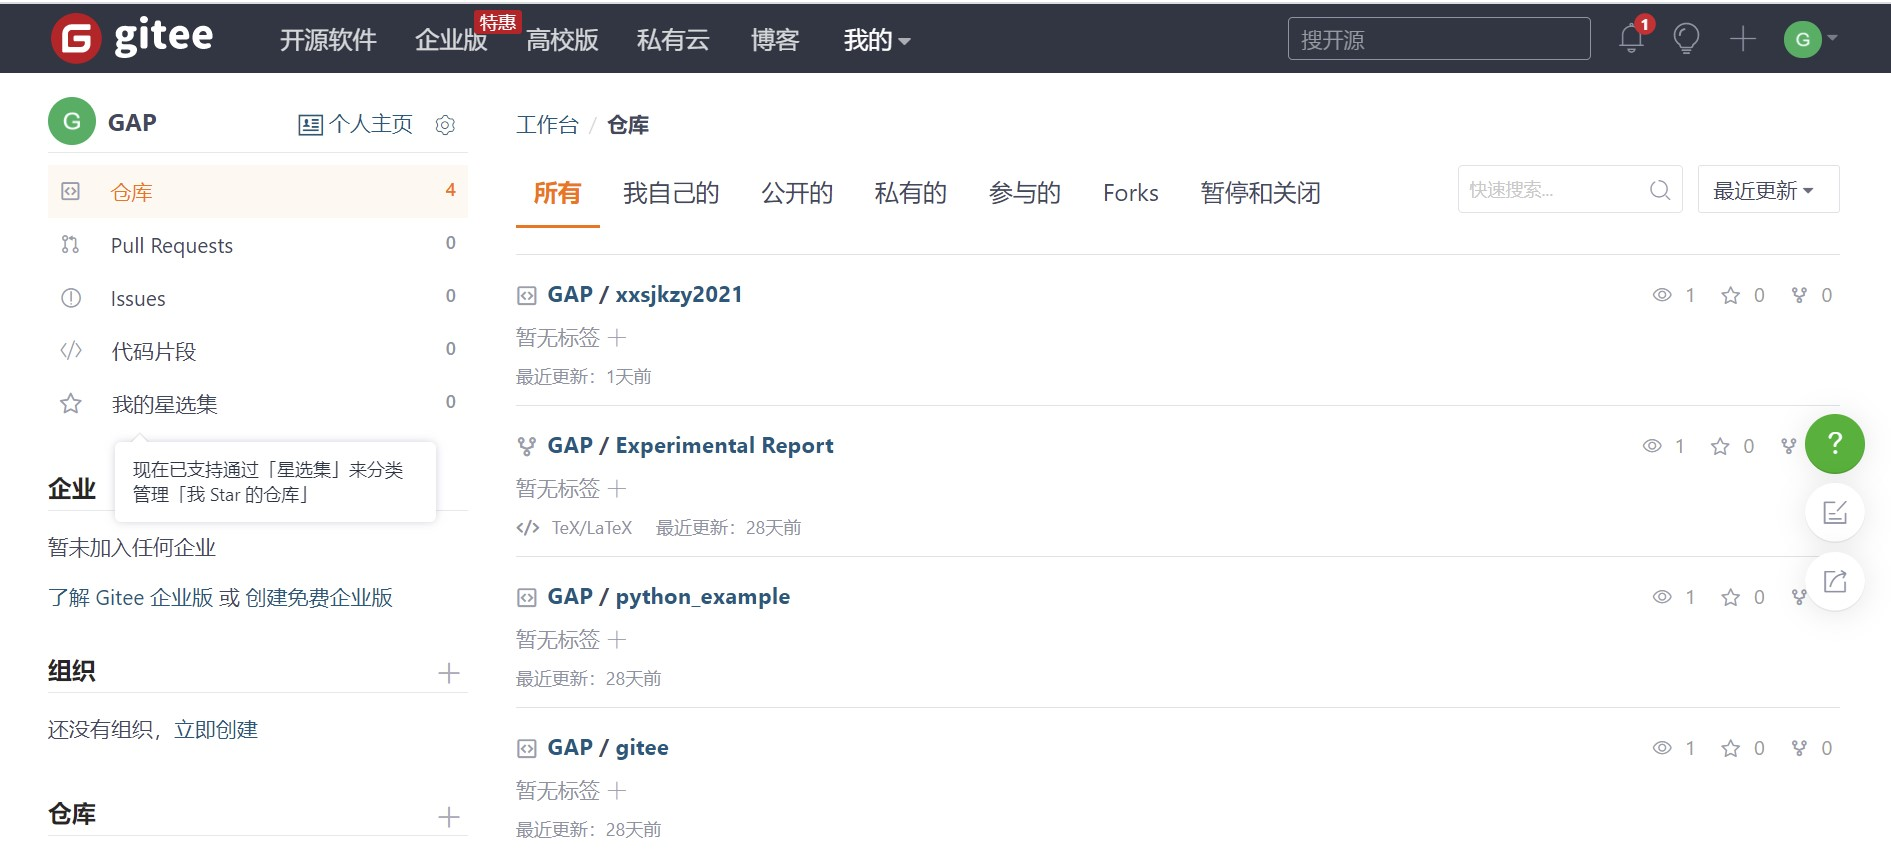
\includegraphics[scale=0.43]{images/5-1.jpg}
			\caption{创建多个仓库}
			\label{fig5-1}
		\end{center}
	\end{figure}
	
	\begin{figure}[htb]
		\begin{center}
			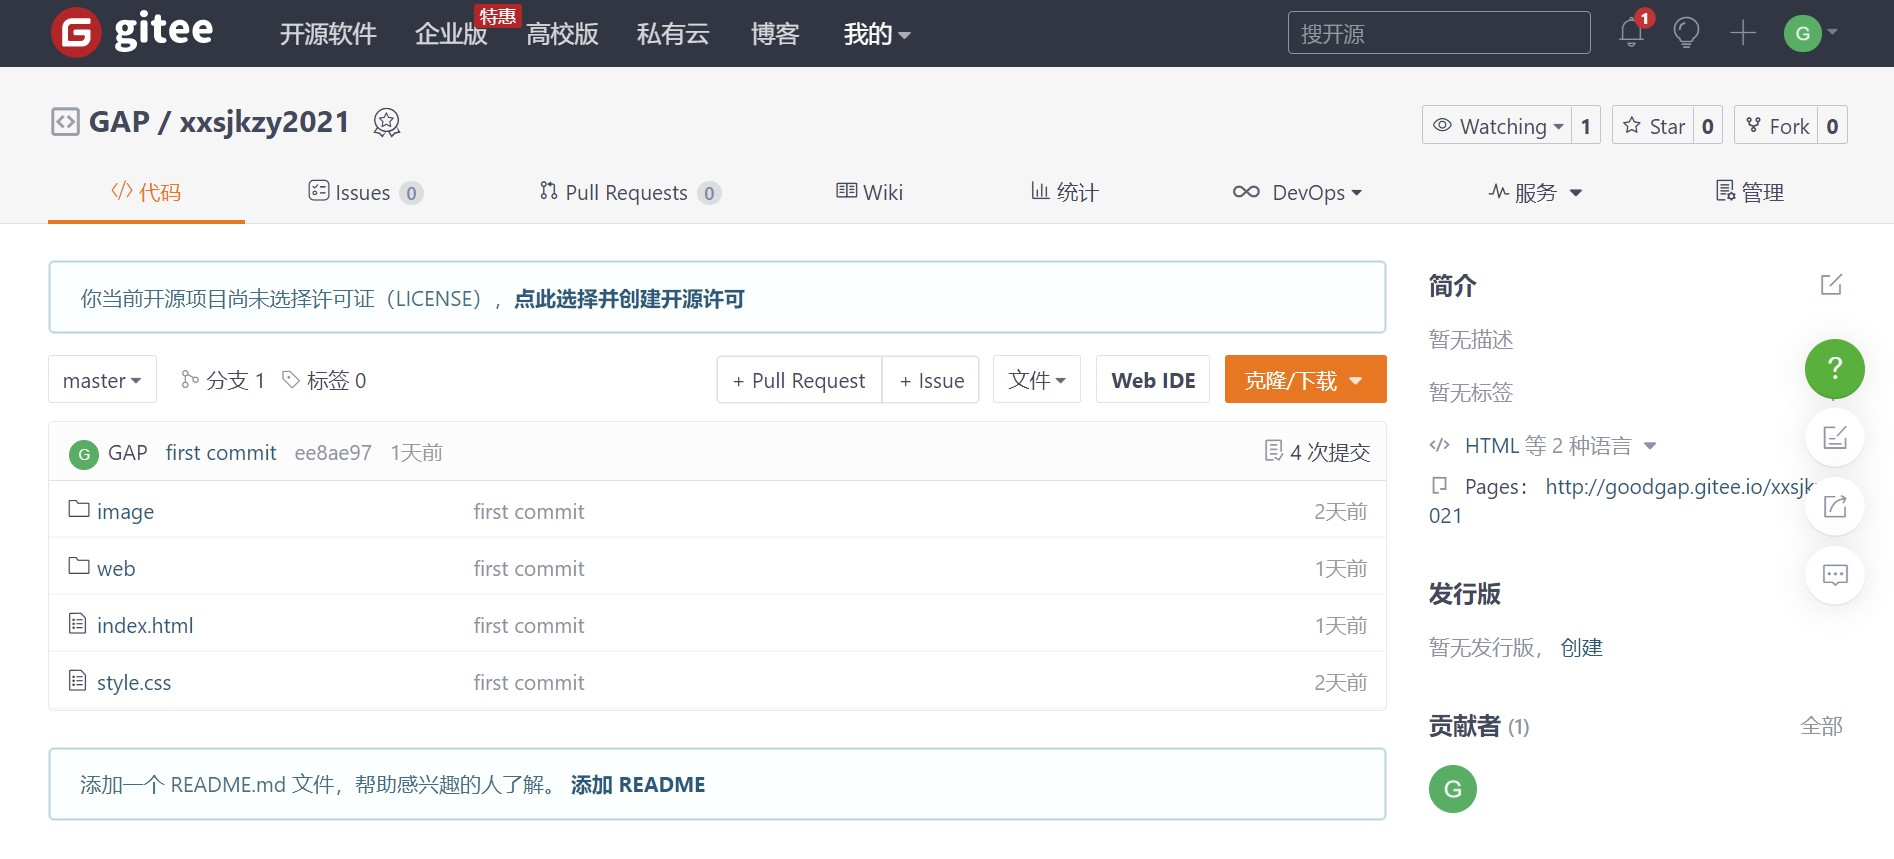
\includegraphics[scale=0.43]{images/5-2.jpg}
			\caption{将本地文件推送到远程仓库}
			\label{fig5-2}
		\end{center}
	\end{figure}

	学习了Git后,我又开辟了一种新的保存代码的方式。这种方式能提高代码文件的安全性,并能轻松地进行代码的分支与合并,功能强大。
	
	\subsection{网页制作Dreamweaver}
	
	在Dreamweaver这一专题中,我学习了如何制作网页,尤其是通过代码的方式实现预期效果,如图\ref{fig6}。
	
	\begin{figure}[htb]
		\begin{center}
			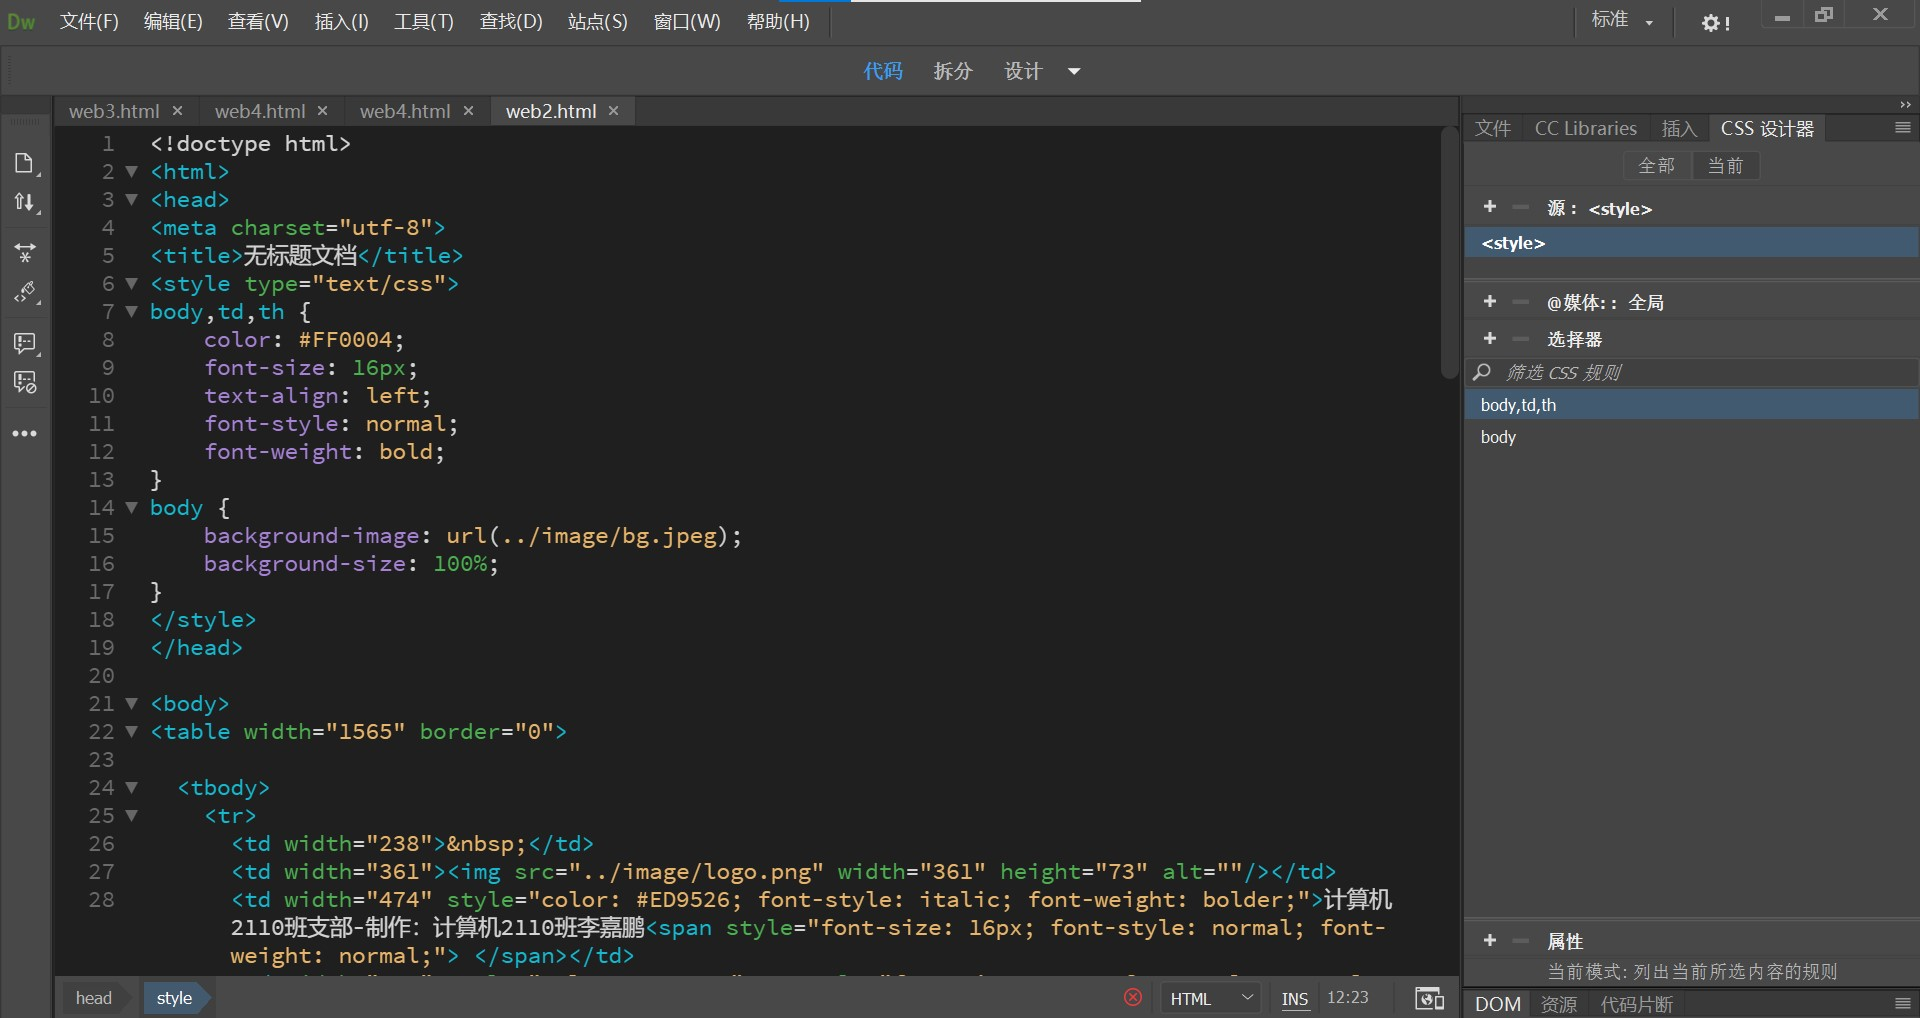
\includegraphics[scale=0.45]{images/6.jpg}
			\caption{利用代码构建网页}
			\label{fig6}
		\end{center}
	\end{figure}
	
	通过课程作业并结合课堂知识,我的网页制作能力得到了极大提高。
	
	
	\nocite{*} %% 作用是不对文献进行引用,但可以生成文献列表
	
	%\bibliographystyle{HustGraduPaper}
	%\bibliography{HustGraduPaper}
	
\end{document}
